\chapter{Related works}
\label{chap:related}

This chapter offers a review of related and comparable studies.
while almost no projects or studies exist at the intersection of all three of these fields, we do find related studies which intersect two of these fields, represented by the edges of \reffig{fig:triangle-model}:
\begin{enumerate}[-]
  \item \refsec{sec:related-geoweb} reviews related works on browser-based geoprocessing
  \item \refsec{sec:related-geovpl} reviews related works on VPLs used for geo-computation
  \item \refsec{sec:related-webvpl} reviews related works on VPL web applications
\end{enumerate}

\section{Browser-based geocomputation}
\label{sec:related-geoweb}

This section is dedicated to related works on client-side geocomputation, or browser-based geocomputation. 
this study prefers to use "browser-based geocomputation" in order to circumvent the ambiguity between native clients like QGIS, and web clients, as described in \refsec{sec:background-web}.

First, a small paragraph on the motivation behind browser based geocomputation.
As stated in \refsec{sec:background-web}, web applications offer safety, distribution and accessibility advantages over native applications.
As such, browser based gis has become a sizable component of the geospatial software landscape. 
% For the average person, an interactive \ac{gis} web application is often their first and only exposure to such a system, be it a web mapping service, a navigation system, or a pandemic outbreak dashboard. 
However, despite the popularity of geographical web applications, the range of actual \ac{gis} abilities these applications have is generally speaking very limited. \ac{geocomputation} is usually not present within the same software environment as the web app. 
This limited range of capabilities inhibits the number of use cases geographical web applications can serve, and with that the usefulness of web \ac{gis} as a whole.
If web applications gain \ac{geocomputation} capabilities, they could grow to be just as diverse and useful as desktop \ac{gis} applications, with the added benefits of being a web application. It would allow for a new range of highly accessible and sharable geocomputation and analysis tools, which end-users could use to post-process and analyze geodata quickly, uniquely, and on demand.

This need has let to the field of Browser-based geocomputation

% NEW PRACTICAL ATTEMPT. WHY? 
% - csg still has a lot of potential
% - previous studies:
%   - are dated
%   - prioritized theory over practicalities
%   - utilized the web's major feature of Accessibility and the clients feature of    
%     Interactivity inadequately 
%   - were not creative enough in terms of possible use-cases 

Browser-based geocomputation has seen some academic interest throughout the last decade \cite{hamilton_client-side_2014, panidi_hybrid_2015, kulawiak_analysis_2019}.

Hamilton et. al. created a 'thick-client', capable of replacing certain elements of server-side geoprocessing with browser-based geoprocessing \cite{hamilton_client-side_2014}. 
At first glance, the results seem unfavorable . 
The paper states how "the current implementation of web browsers are limited in their ability to execute JavaScript geoprocessing and not yet prepared to process data sizes larger than about 7,000 to 10,000 vertices before either prompting an unresponsive script warning in the browser or potentially losing the interest of the user."(SOURCE). 
While these findings are insightful, they are not directly applicable to the efforts of this study proposal. Three reasons for this:

\begin{itemize}
  \item The paper stems from 2014. Since then, web browsers have seen a significant increase in performance thanks to advancements in JavaScript JIT compilers \cite{haas_bringing_2017, kulawiak_analysis_2019}. 
  \item The paper does not use compile-time optimizations. The authors could have utilized 'asm.js' \cite{mozilla_asmjs_2013} which did exist at the time. 
  \item The paper uses a javascript library which was never designed to handle large datasets.
\end{itemize}

The same statements can be made about similar efforts of Panidi et. al. \cite{panidi_hybrid_2015}. 
However, Panidi et. al. never proposed browser-based geoprocessing as a replacement of server-side geoprocessing. 
Instead, the authors propose a hybrid approach, combining the advantages of server-side and browser-based geoprocessing. 
They also present the observation that browser-based versus server-side geoprocessing shouldn't necessarily be a compassion of performance. 
"User convenience" as they put it, might dictate the usage of browser-based geoprocessing in certain situations, despite speed considerations \cite{panidi_hybrid_2015}. 

This concern the general web community would label as \ac{ux}, is shared by a more recent paper \cite{kulawiak_analysis_2019}. 
Their article examines the current state of the web from the point of view of developing cost-effective Web-GIS applications for companies and institutions. 
Their research reaches a conclusion favorable towards browser-based data processing: "[Client-side data processing], in particular, shows new opportunities for cost optimization of Web-GIS development and deployment. 
The introduction of HTML5 has permitted for construction of platform-independent thick clients which offer data processing performance which under the right circumstances may be close to that of server-side solutions. 
In this context, institutions [...] should consider implementing Web-GIS with client-side data processing, which could result in cost savings without negative impacts on the user experience.".

% Based on the topic of client-side geospatial processing, we can state that web technologies contain a very dynamic temporal component. All research can become outdated, but performance analysis of web technologies are especially quick to change.  

From these papers we can summarize a true academic and even commercial interest in browser based geoprocessing over the last decade. 
However, practical implementation details remain highly experimental, or are simply not covered.  
The implementations of \cite{panidi_hybrid_2015, hamilton_client-side_2014} were written in a time before WebAssembly \& major javascript optimizations, and the study of \cite{kulawiak_analysis_2019} prioritized theory over practice. 
Additionally, to the best of the authors's knowledge, all papers concerned with browser-based geoprocessing either tried to use existing JavaScript libraries, or tried to write their own experimental WebAssembly / JavaScript libraries. 
No studies have been performed on the topic of compiling existing C++/Rust geoprocessing libraries to the web. 

%%%%%%%%%%%%%%%%%%%%%%%%%%%%%%%%%%%%%%%%%%%%%%%%%%%%%%%%%%%%%%%%%%%%%%%%%%%%%%%
\subsubsection*{Commercial web-based geocomputations software}
Despite the earlier statement of the general lack of \ac{geocomputation} within browsers, there are exceptions. 
A select number of web-based \ac{gis} applications are starting to experiment with empowering end-users with geocomputation. 
These applications will briefly be mentioned.
 
% https://geotiff.io/
GeoTIFF (SOURCE, \reffig{fig:geotiff}), is a web-based geoTIFF processing tool, and fully open source. 
It offers basic operations such as taking the median or \& mean of a certain area, color band arithmetic, and can plot histograms, all calculated within the browser using customly written javascript libraries.

\begin{figure}
  \centering
  \graphicspath{ {../../assets/images/background/geo-web/} }
  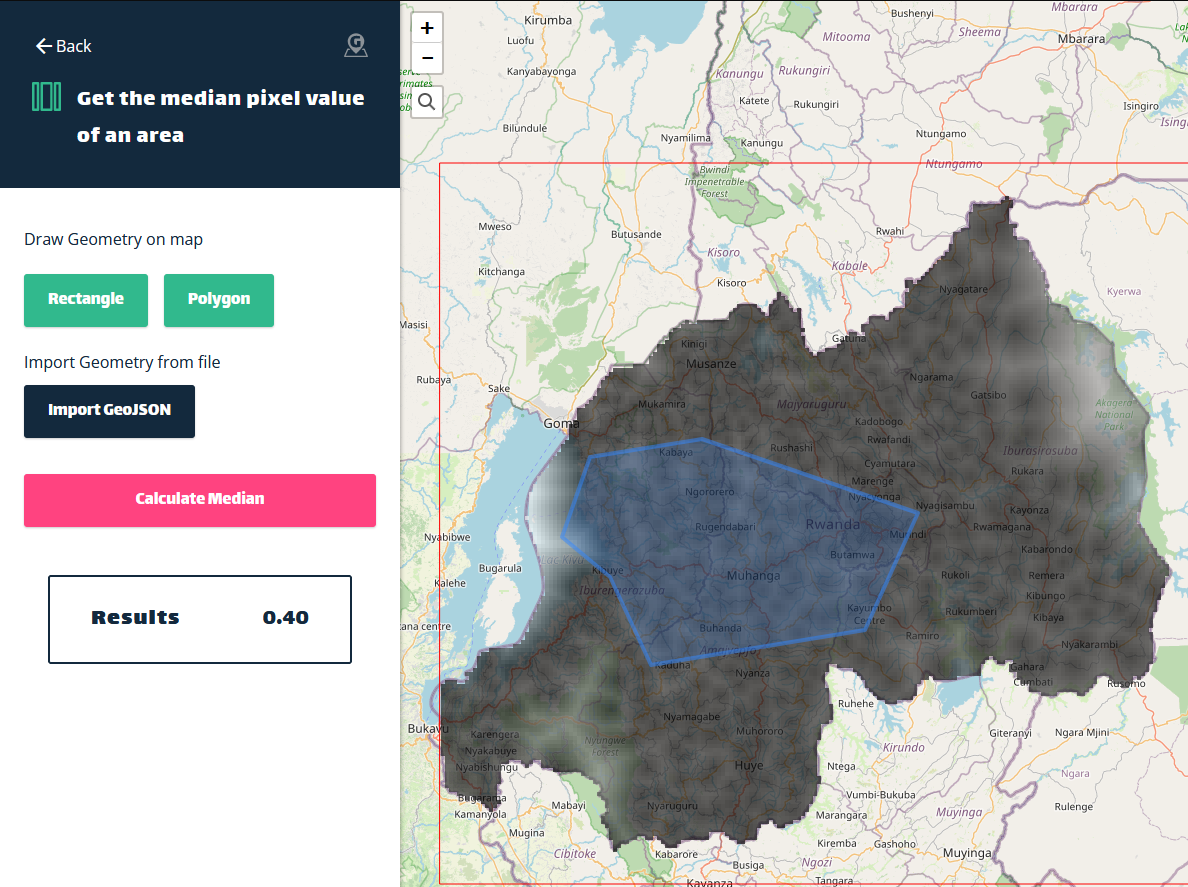
\includegraphics[width=270px]{geotiff.png}
  \caption{The geoTIFF.io application}
  \label{fig:geotiff}
\end{figure}


\begin{figure}
  \centering
  \graphicspath{ {../../assets/images/background/geo-web/} }
  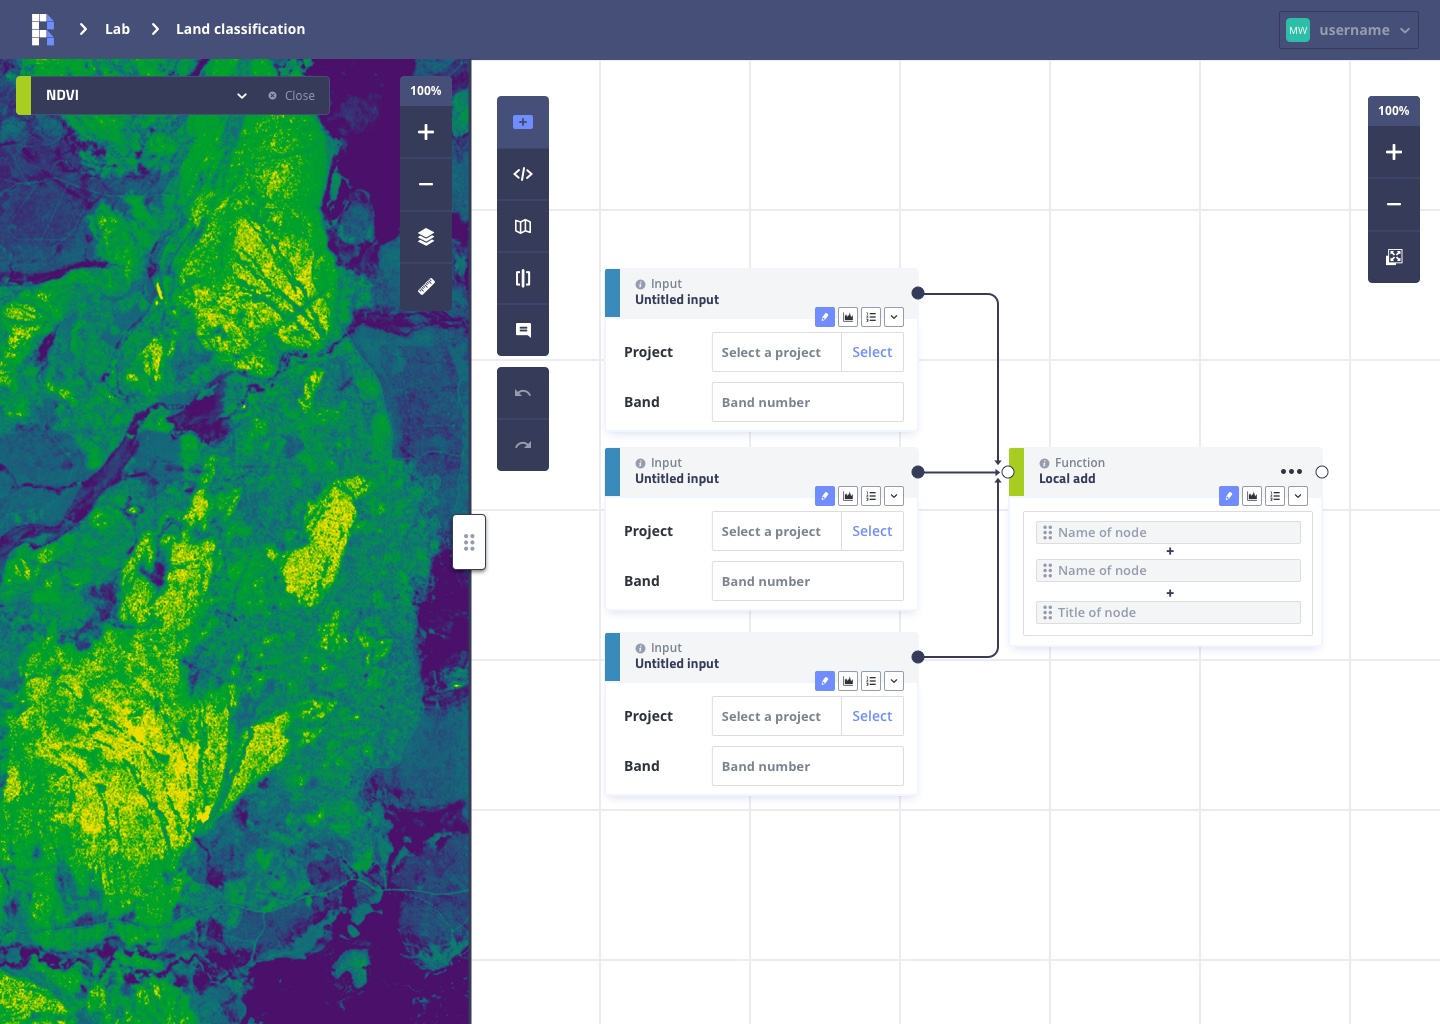
\includegraphics[width=270px]{rasterfoundry-2.jpg}
  \caption{The ModelLab application}
  \label{fig:modellab}
\end{figure}

% https://www.eclipse.org/community/eclipse_newsletter/2018/december/geotrellis.php 
% https://www.azavea.com/blog/2016/09/26/raster-foundry-model-lab-phase-ii-sbir/
Azavea's Raster Foundry and ModelLab (Powered by GeoTrellis), is another GeoTIFF / raster based web processing tool, in which basic queries and calculations are possible (SOURCE). 
This tool offers more advanced types of geocomputation, like buffering / minkowski sums, and even multi-stage processing via a simple but clear visual programming language (see \reffig{fig:modellab}). 
% There reasoning: "Widespread access to frequent, high-resolution Earth observation imagery has created the need for innovative tools like ModelLab that will 
However, the tool uses mostly server-side processing, making this application less relevant to this study. 

Also, despite their mission statement to: "help individuals and organizations to effectively access, analyze, edit, and visualize remotely sensed data in transformative new ways without years of specialized training or ongoing investments in proprietary software and technology infrastructure."(Source), The tool appears to be reliant on their own proprietary infrastructure to save and run the application.
The author of this study was also not able to find a public demo of the application. 

\begin{figure}
  \centering
  \graphicspath{ {../../assets/images/background/geo-web/} }
  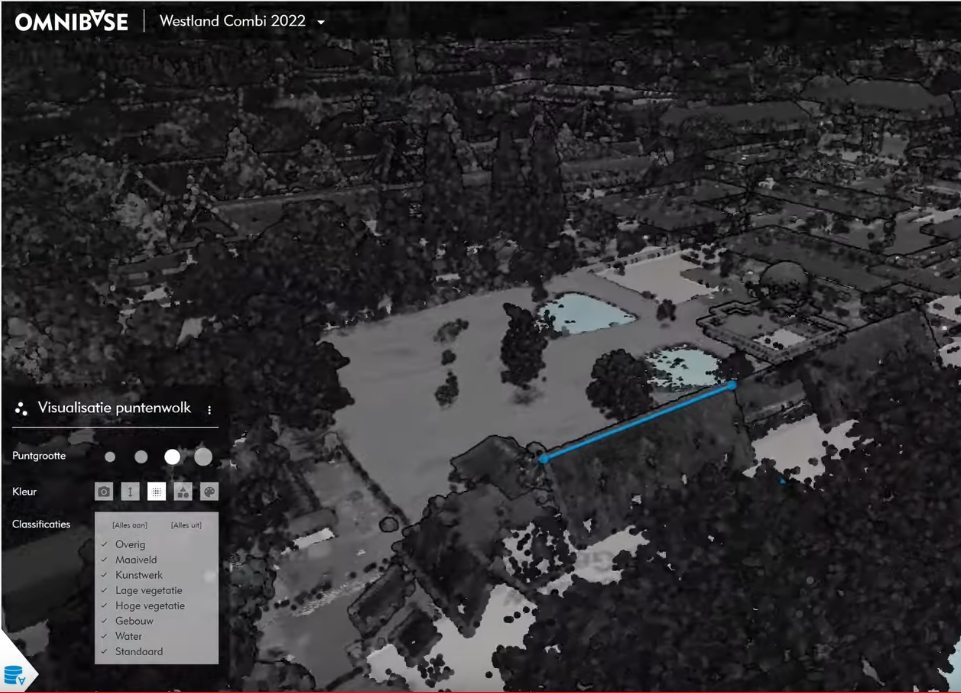
\includegraphics[width=270px]{omnibase.png}
  \caption{The Omnibase application}
  \label{fig:omnibase}
\end{figure}

The last web-based geocomputation platform this study would like to mention is Geodelta's Omnibase application (SOURCE: GEODELTA, \reffig{fig:omnibase}). 
Omnibase is a 3D web \ac{gis} application for viewing and analyzing pointclouds and areal imagery datasets.
It offers client-side geocomputation in the form of measuring distances between locations, and calculating the area of a polygon.  
It also offers photogrammetry-techniques such as forward incision of a point in multiple images, but these are calculated server-side. 

% - https://openscad.org/


%%%%%%%%%%%%%%%%%%%%%%%%%%%%%%%%%%%%%%%%%%%%%%%%%%%%%%%%%%%%%%%%%%%%%%%%%%%%%%%
%%%%%%%%%%%%%%%%%%%%%%%%%%%%%%%%%%%%%%%%%%%%%%%%%%%%%%%%%%%%%%%%%%%%%%%%%%%%%%%
%%%%%%%%%%%%%%%%%%%%%%%%%%%%%%%%%%%%%%%%%%%%%%%%%%%%%%%%%%%%%%%%%%%%%%%%%%%%%%%

%  \subsection*{The Cloud Native Geospatial movement}

% ( Not sure if I wanna go there... )

% % Establish OGC in two sentences, mentioning their name and Vision
% The Open Geospatial Consortium (OGC)...
% Mission: FAIR Geodata 

% % Establish Cloud Native movement.
% % GIS as one big LAN party
% A prominent development within the OGC is the recent effort towards a \textbf{"Cloud Native Geospatial"} future. 
% This initiative aims to radically simplify geodata storehouses to static servers serving large, singular binary geodata files. All processing and analysis of this geodata can then be performed by separate cloud-based web services. 
% This architecture has many advantages over current geodata storage and analysis methods:
% \begin{itemize}
%   \item These new Cloud Native geodata formats are much cheaper to access by front-end and back-end services, compared to active services.
%   \item Substituting active SQL or noSQL databases by static binary files is easier and cheaper for data providers, leading to more and more readily available geodata.
%   \item By using supercomputers (Microsoft Planetary Computer) and cloud-storage (AWS), Geodata processes could make use of near-infinite computational and storage resources. 
%   \item By having all data centralized in one location or type of location, new, large scale patterns within our geodata could be discovered.  
%   \item For web GIS, this would offer direct data streaming options, similar to services like "Netflix" or "Spotify".  
% \end{itemize}

% These features may have a far reaching impact on society. Chris Holmes, forerunner of the cloud-native geospatial movement, envisions what the movement could mean for even non-GIS users: 
% \emph{
%   With the introduction of accessible, centralized data, and the dramatically different workflows that follow, Cloud Native Geospatial has the potential to introduce new, non-specialized users to the power of geospatial information that GIS practitioners have enjoyed for decades. [...]. The ecosystem of geospatial experts will collaborate to create analyses and insight, but any non-expert user will be able to select and apply those to the geographic area they care about. \~ Chris Holmes
% }
% % This is also reflected by cloud-native based tools like (Google Earth Engine or RasterFoundry) may achieve such a feed, by being web based and stuff...
% All these reasons explain why the OGC and many other parties are now actively pursuing this vision.

% But while this vision is in active development, many large-scale challenges are still in its way. 
% One of the most important challenges is the required paradigm shift within geo-computation / geoprocessing workflows. 
% The current, common geo-computation workflow of retrieving online data, only to run it through a local process and send the resulting data back into servers, will have to be reversed: In a cloud-native future, we will not retrieve data for our local process, but we will upload our process to the data.  
% This introduces a sizable challenge: \textbf{Portable, Containerized Geo-computation}.

% % \textbf{and the algorithms powering the processing can be shared online and customized collaboratively}. -> Chris again

% % \begin{itemize}
% %   \item Up to this point, the world of GIS has done a considerable effort to make geodata more Findable, Accessible, Interoperable, and Reusable. The challenge of Portable geo-computation now forces us to extend the effort of FAIR geodata to FAIR geodata computation as well.  
% %   \item If we want our geodata processes to be just as portable as the geodata it takes as input, then perhaps the FAIR paradigm should extend from FAIR geodata to FAIR geodata processing . FAIR geo-computation.
% %   \item Furthermore, it remains a mystery how these containerized containerized processes will be configured and accessed by frontend computation environments. 
% %   \item Holmes: one of the vital ingredients: \emph{"and the algorithms powering the processing can be shared online and customized collaboratively"}.
% % \end{itemize}

% The challenge of sharing and chaining together containerized fragments of geoprocesses to a variety of environments will require more than just open source collaboration. 
% This study interprets the challenge of portable geo-computation by means of the FAIR paradigm. 
% If geodata processes need to be just as portable as the geodata forming the input and output, then perhaps the FAIR paradigm should extend from FAIR geodata to FAIR geodata \emph{processing} as well.
% The challenge facing the cloud-native vision then becomes: \textbf{How to make geo-computation Findable, Accessible, Interoperable, and Reusable?} 
% This links back to containerization, for containerization is a very powerful method of making geo-computation more Interoperable and Reusable.

% % state of the art regarding this issue, make a path towards the particular thesis, and why it is an application
% The current state of the art is far removed from either portable or FAIR geo-computation. 
% \todo{Improve this intro}
% \begin{itemize}
%   \item current methods: Docker, and some geo-computation platforms.
%   \item Not many implementations using WebAssembly, while this is a prime candidate: Even the guy who made Docker said so. 
%   \item ignore the cloud: focus on the act of containerizing geoprocesses using webassembly an sich
% \end{itemize}

\section{Visual programming and geocomputation}
\label{sec:related-geovpl}

This section is dedicated to giving an overview of related works on \ac{vpl}s related to geocomputation.

\begin{note}
  [I just wish to state: "these applications exist".
  I also wish to make some comments on the interplay between geocomputation and vpl. 
  Are these fields complimentary?
  These will also be referred back to during the methodology chapter]    
\end{note}

\reffig{fig:geovpl:table} offers this overview of some of the more significant \ac{vpl}s present in not only \ac{gis}, but also the neighboring domains based on computer graphics.
Why these fields are regarded as relevant are explained in \refsec{sec:background-geo}. 

\begin{figure}
  \centering
  \graphicspath{ {../../assets/tables/} }
  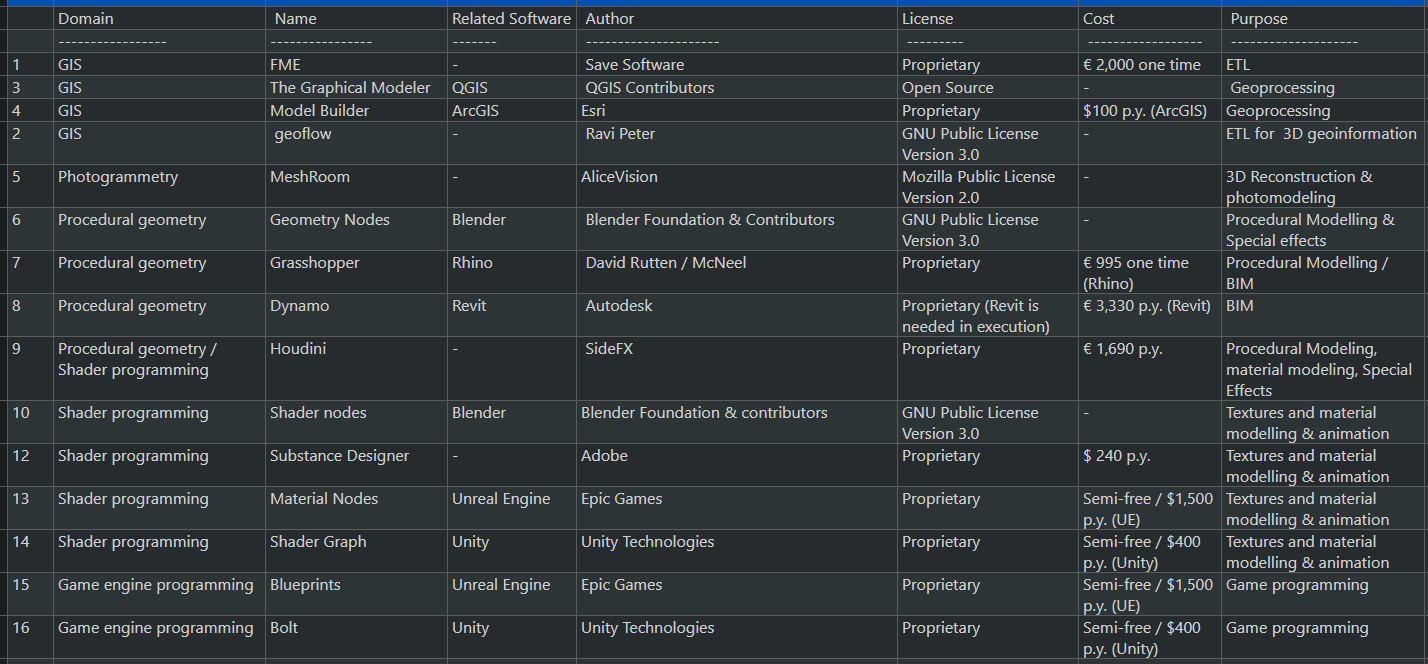
\includegraphics[width=400px]{geovpl.png}
  \caption{An overview of VPLs in the field of GIS and adjacent domains}
  \label{fig:geovpl:table}
\end{figure}

\subsection*{ VPLs in GIS }

Within the field of geo informatics, \ac{vpl}s are not a new phenomenon. VPLs have been used for decades to specify geodata transformations and performing spatial analyses.  

By far the most well-known visual programming language within the field of \ac{gis} is the commercial \ac{etl} tool FME (Source, \reffig{fig:gisvpl:1}). 
This tool is widely used by \ac{gis} professionals for extracting data from various sources, transforming data into a desired format, and then loading this data into a database, or just saving it locally.  
FME is most often used within GIS to harmonize heterogenous databases, and as such specializes in tabular datasets. 

The two major GIS applications ArcGIS and QGIS also have specific \ac{vpl}s attached to their applications. 
The main use-case for these \ac{vpl}s is to automate repetitive workflows within ArcGIS or QGIS. 

Lastly, Geoflow is a much newer \ac{vpl} meant for generic 3D geodata processing.
While this application is still in an early phase,  it already offers very powerful 
range of functions.
It offers CGAL processes like alpha shape, triangulation and line simplification, as well as direct visualization of in-between products.

% In comparison with the three aforementioned \ac{GIS} vpls, geoflow is much richer 

\begin{figure}
\centering
\begin{subfigure}[b]{0.45\linewidth}
  \graphicspath{{../../assets/images/background/geo-vpl/}}
  \centering
  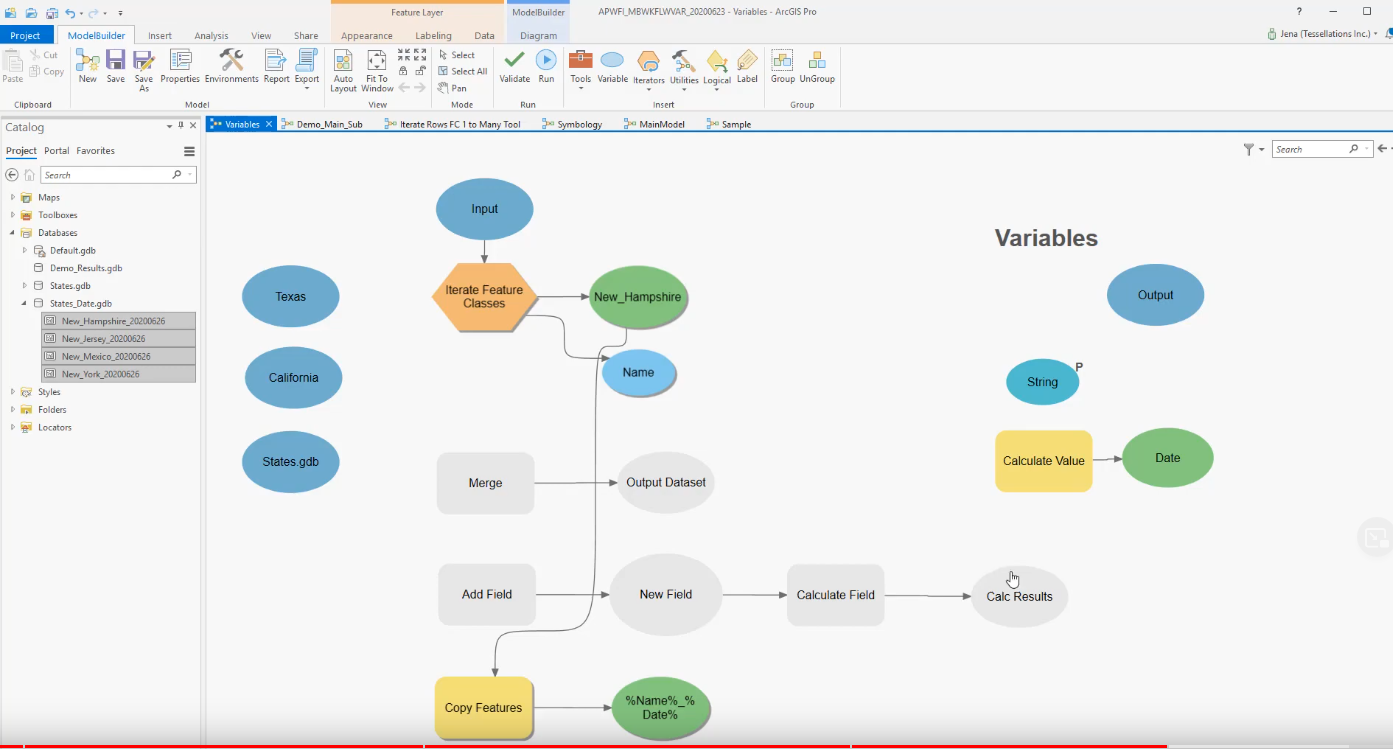
\includegraphics[width=\linewidth]{arcgis.png}
  \caption{}\label{fig:gisvpl:1}
\end{subfigure}%
\qquad 
\begin{subfigure}[b]{0.45\linewidth}
  \graphicspath{{../../assets/images/background/geo-vpl/}}
  \centering
  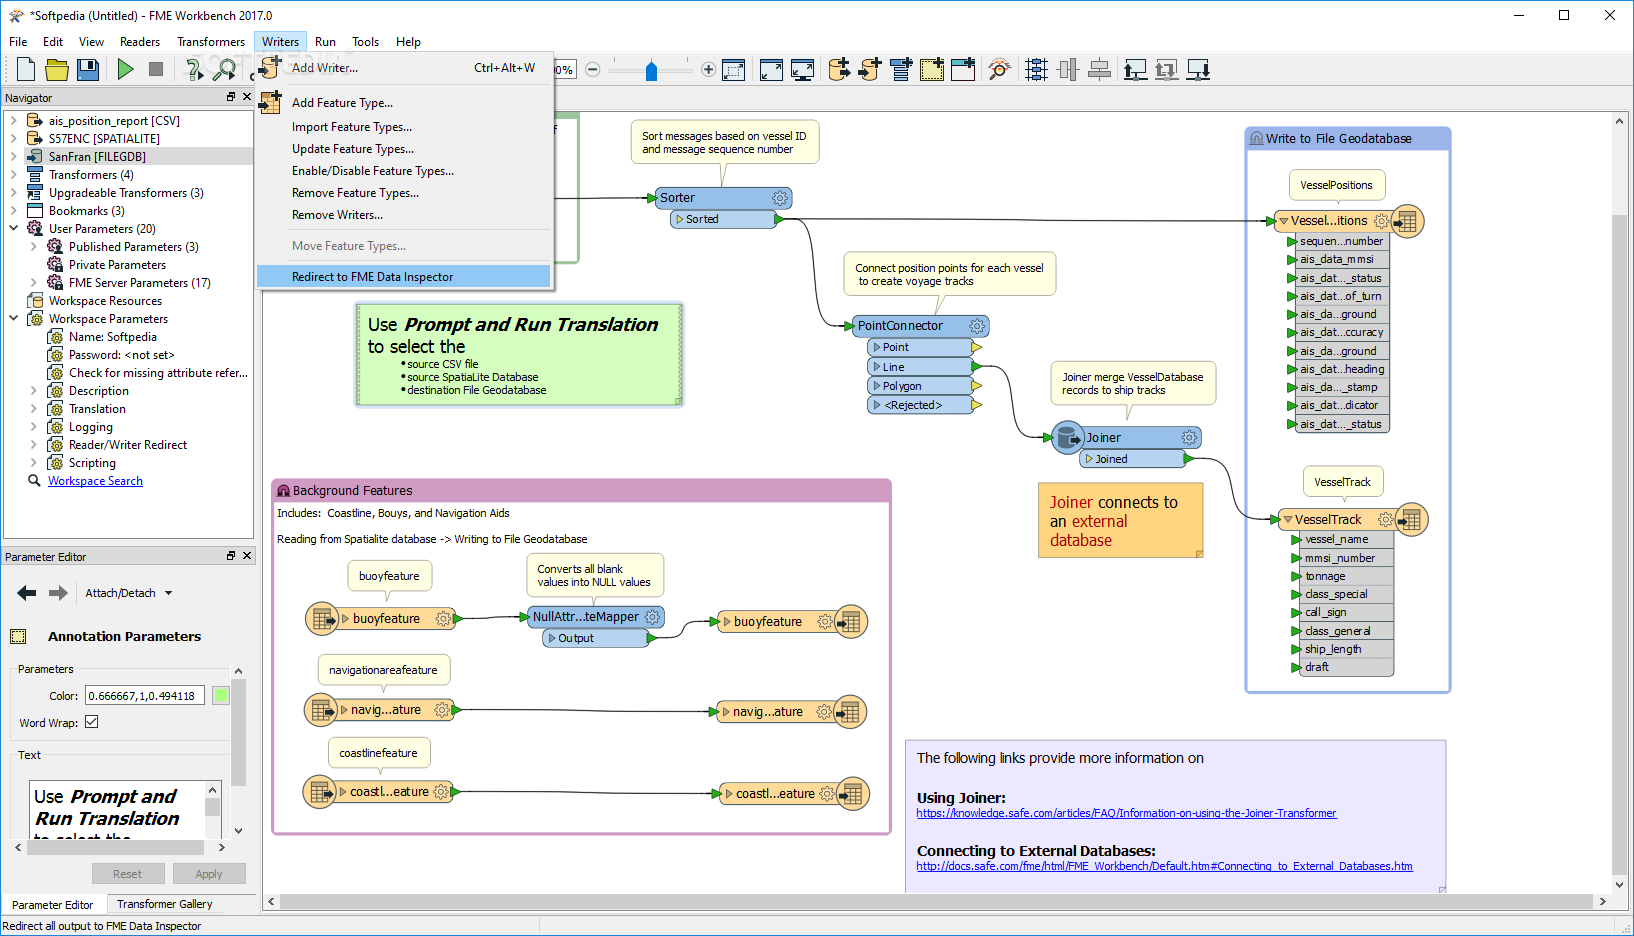
\includegraphics[width=\linewidth]{fme.png}
  \caption{}\label{fig:gisvpl:2}
\end{subfigure}%
\\
\begin{subfigure}[c]{0.45\linewidth}
  \centering
  \graphicspath{{../../assets/images/background/geo-vpl/}}
  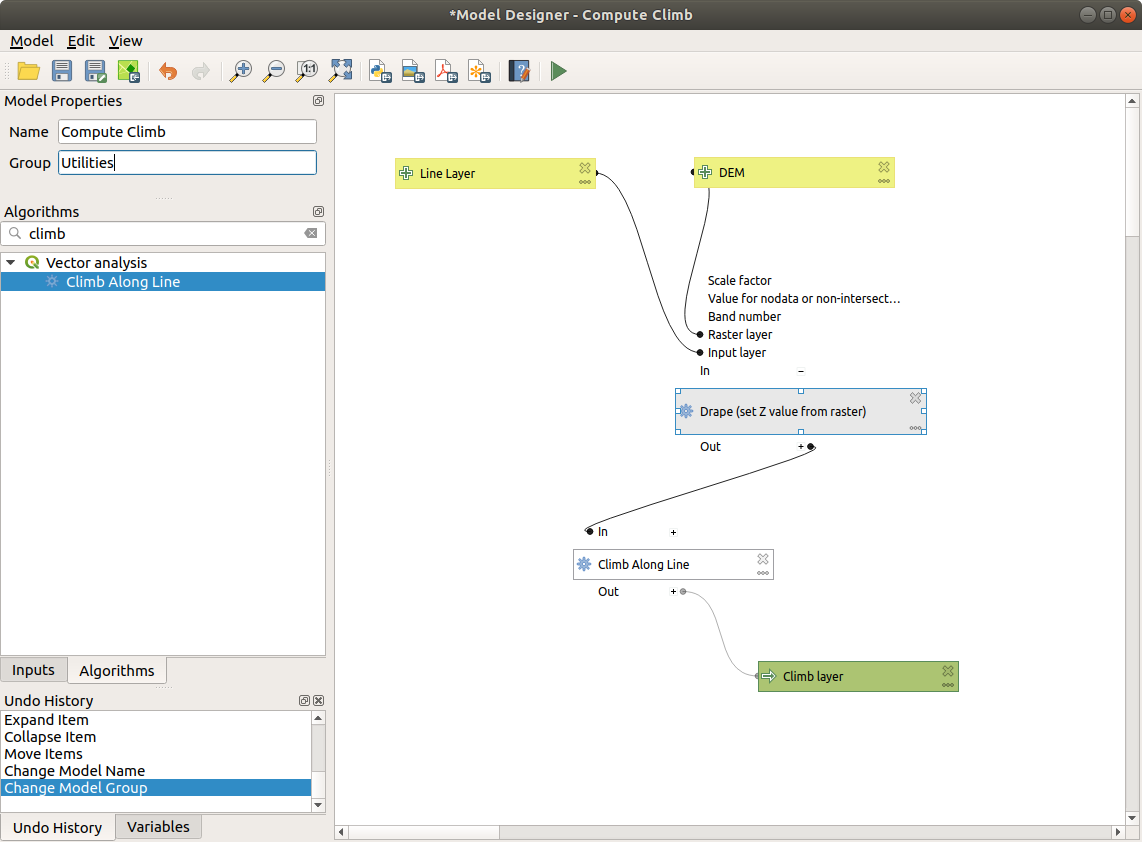
\includegraphics[width=\linewidth]{qgis.png}
  \caption{}\label{fig:gisvpl:3}
\end{subfigure}%
\qquad 
\begin{subfigure}[d]{0.45\linewidth}
  \centering
  \graphicspath{{../../assets/images/background/geo-vpl/}}
  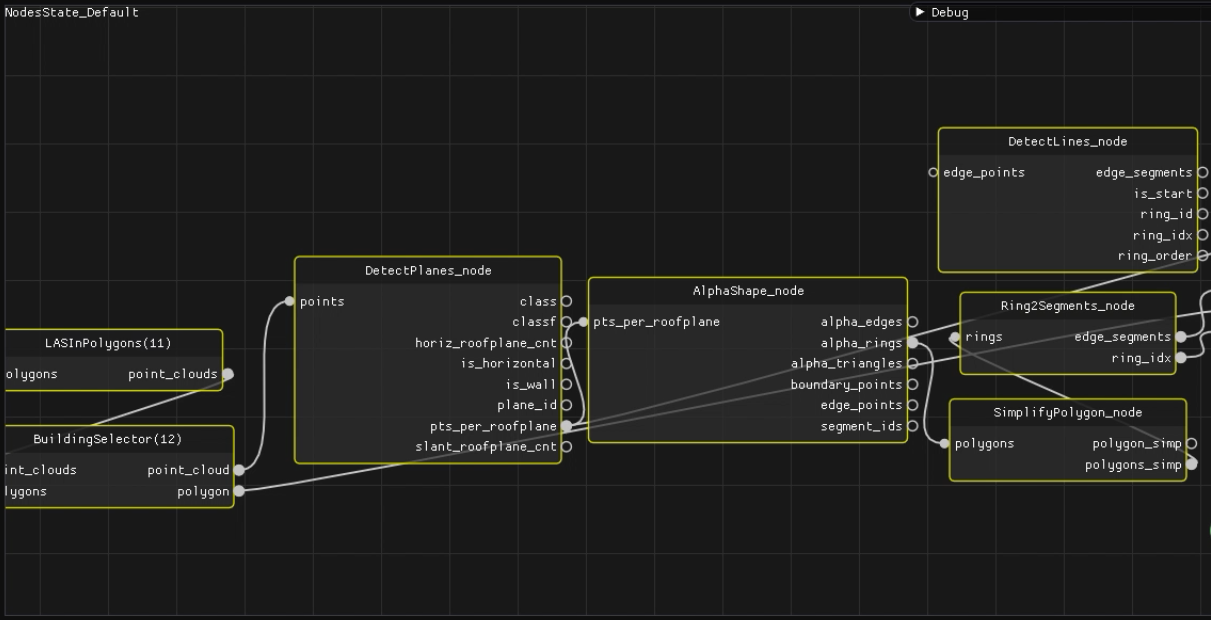
\includegraphics[width=\linewidth]{geoflow.png}
  \caption{}\label{fig:gisvpl:4}
\end{subfigure}%
\caption[GIS VPLs]{Four VPLs used in the field of GIS: ArcGIS's Model Builder (a), Save Software's FME (b), QGIS's Graphical Modeler (c), and Geoflow (d).}
\label{fig:gisvpl}
\end{figure}

\subsection*{ VPLs in neighboring domains }

\reffig{fig:geovpl:table} shows a great number of non-GIS \ac{vpl}s.
while these do not explicitly cover GIS, their close ties to computer graphics are still highly relevant to GIS and the activity of geocomputation.  

The choices of which vpl to include in \reffig{fig:geovpl:table} are based upon popularity.  
The particular ones chosen see a lot of use, evident by the sheer number of courses and tutorials which cover these vpls, and the popularity of the software packages these applications are attached to. 
In fact, many of the mentioned vpls are popular enough that it is safe to say that \ac{vpl}s are common in the wider field of computer graphics. 
This study limits itself to four sub-domains relevant to geocomputation:
\begin{itemize}[-]
  \item VPLs to calculate materials, shaders and textures
  \item VPLs to calculate geometry
  \item VPLs to perform photogrammetry reconstruction. 
  \item VPLs to calculate behavior and logic
\end{itemize}

\subsubsection*{Commonalities}
One interesting fact is that we see a great number of parallels among all these \ac{vpl}s.
\begin{itemize}[-]
  \item All are diagram-based vpls.
  \item All offer inspection of in-between products. Some even visualize data being parsed between nodes.
  \item All emphasize a process of "parametrization": with sliders and other UI elements, the vpls seem to be intended for rapid experimentation.
\end{itemize}
Moreover, the persistence of visual programming within these computer graphics fields, suggests that visual programming languages are advantageous for calculations dealing with 2D and 3D data.
This might be because all these vpls, with exception to the behavior vpls, are essentially dealing with "production pipelines".
No networking, no distributed systems, just one calculation from start to finish, to produce a desired product.  
However, the sheer amount of possible steps within these pipelines, together with the challenges of fine-tuning many relevant parameters, and the importance of inspecting in-between products visually, do not allow these pipelines to be configured by conventional UI's. 
Therefore, the \ac{vpl} might be a perfect fit for all 2D and 3D data pipelines.
vpls allow rapid debugging, rapid experimentation, and the straight-forward nature of 2D/3D pipelines mitigate the challenge vpls have with representing imperative flow statements (\m{if, else, for, while, break}). 

\subsubsection*{Material VPLs}
By far the most commonplace type of vpl present in computer graphics are material Vpls. 
In this context, the concept "material" often refers to a combination of 2D textures and shaders. 
These include PBR settings, normal maps, bump maps, and / or custom shader programs. 
The repetitive and time-consuming nature of manually creating textures, and the fact that some of these material properties can be inferred from each other, lead many CG applications to develop \ac{vpl}s. 
3D artists can now use these \ac{vpl}s to create procedural textures.

\begin{figure}
\centering
\begin{subfigure}[b]{0.45\linewidth}
  \graphicspath{{../../assets/images/background/geo-vpl/}}
  \centering
  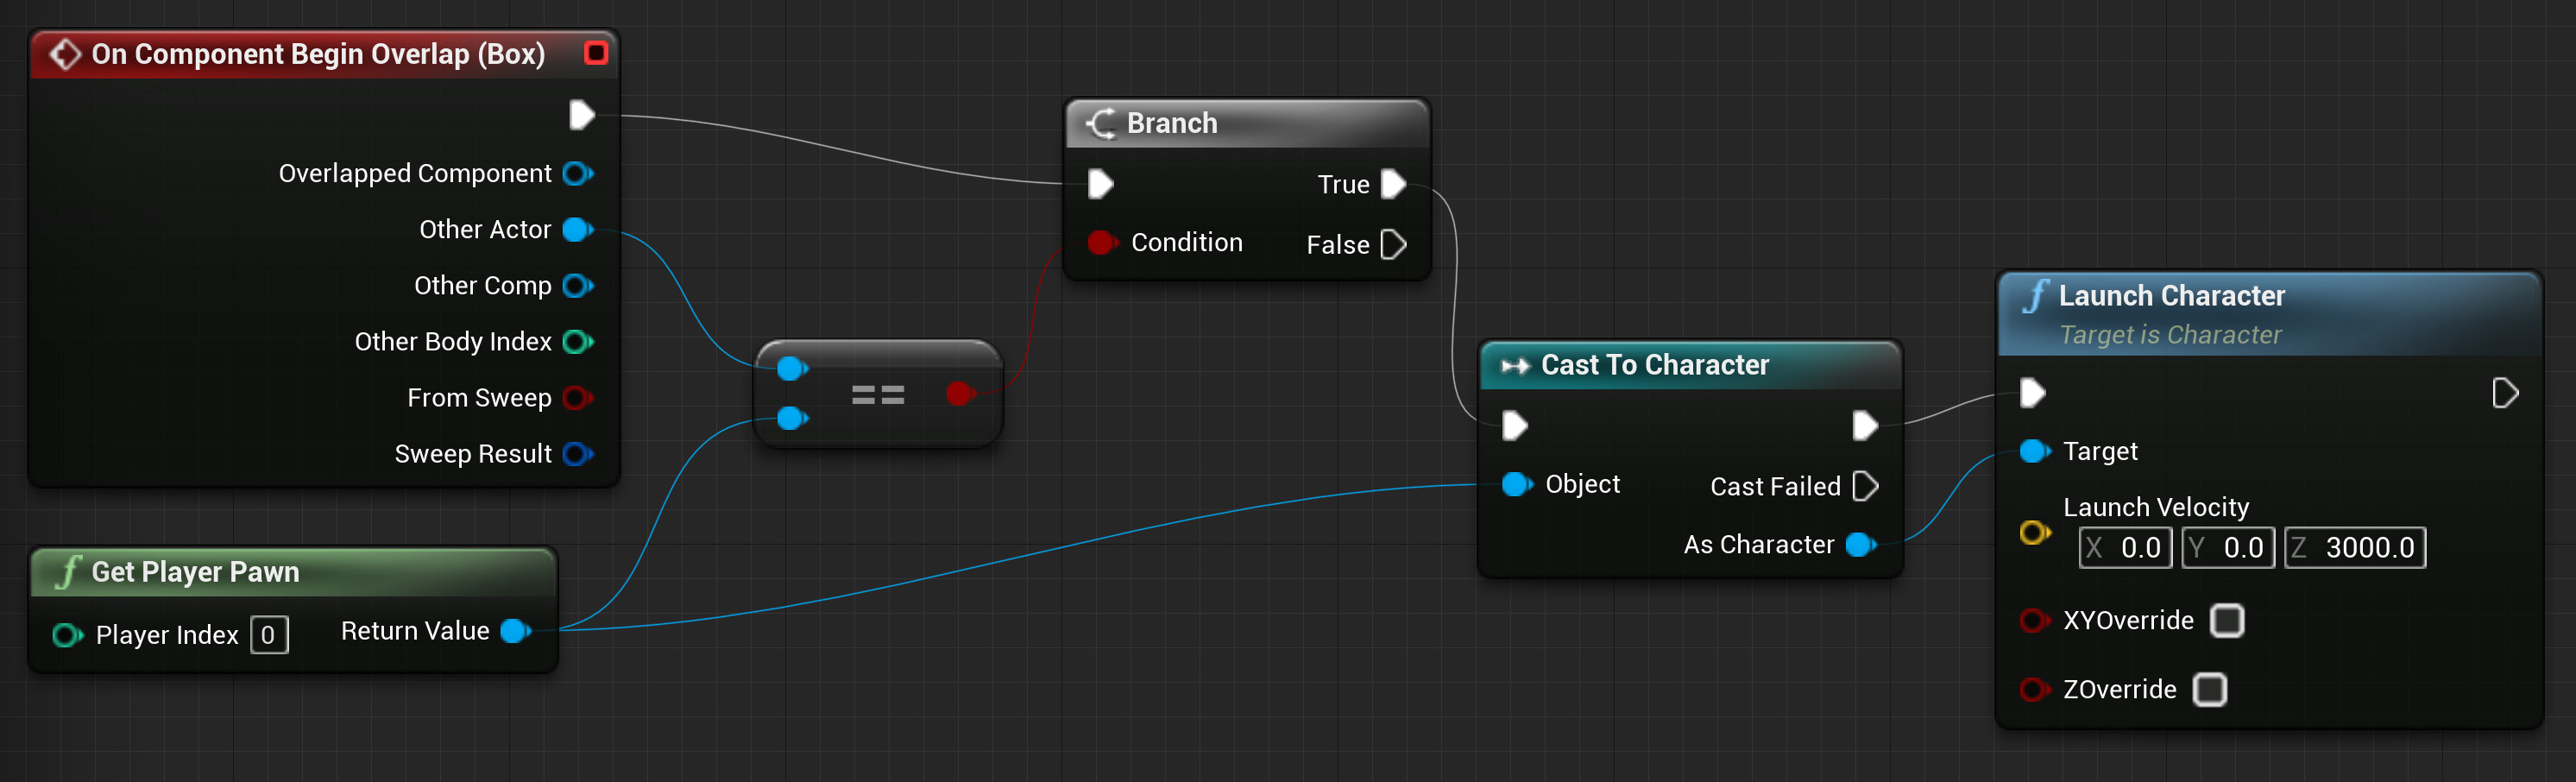
\includegraphics[width=\linewidth]{unreal-blueprints.jpg}
  \caption{}\label{fig:texture-vpl:1}
\end{subfigure}%
\qquad %-- that adds some space between th 2 figures
\begin{subfigure}[b]{0.45\linewidth}
  \graphicspath{{../../assets/images/background/geo-vpl/}}
  \centering
  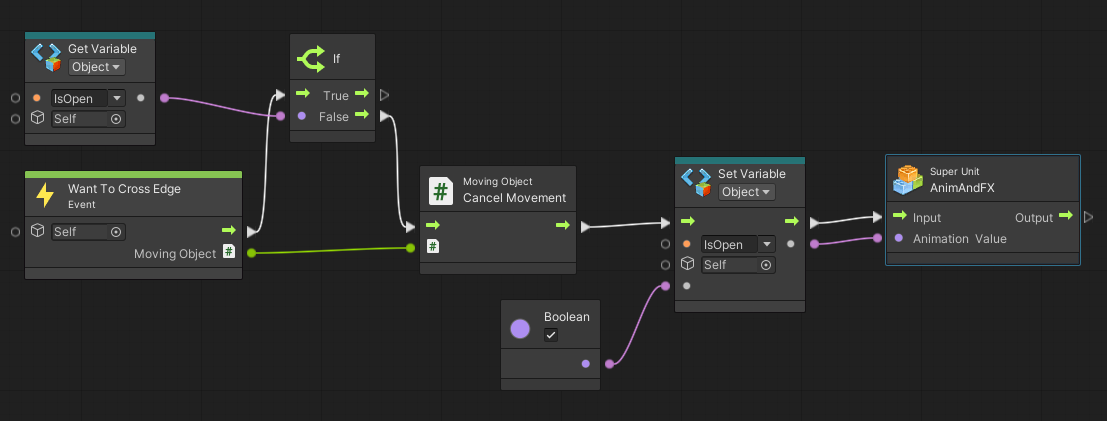
\includegraphics[width=\linewidth]{unity-bolt-2.png}
  \caption{}\label{fig:texture-vpl:2}
\end{subfigure}%
\caption[Texture VPLs]{TODO: add texture vpls}
\label{fig:texture-vpl}
\end{figure}
    
\subsubsection*{Geometry, and photogrammetric VPLs}

Procedural Geometry \ac{vpl}s are not far behind the material \ac{vpl}s in terms of popularity.
Applications like Blender's geometry nodes, Rhino's Grasshopper, or Houdini, are all widely used to automate the creation of geometry. 
Where Houdini and Blender's vpls are primarily used in games and special effects, Grasshopper sees much usage in the Architecture, Engineering and construction industry. In this field, procedural geometry is often referred to as "parametric design".

Alicevision's Meshroom application must also be mentioned.
While this can be regarded as procedural modelling, the complexity and computation involved in photogrammetry make a vpl offering it a class in of itself. 
The vpl inside of Meshroom can be used to fine tune all stages of the 3D reconstruction process.

\begin{figure}
  \centering
  \begin{subfigure}[b]{0.45\linewidth}
    \graphicspath{{../../assets/images/background/geo-vpl/}}
    \centering
    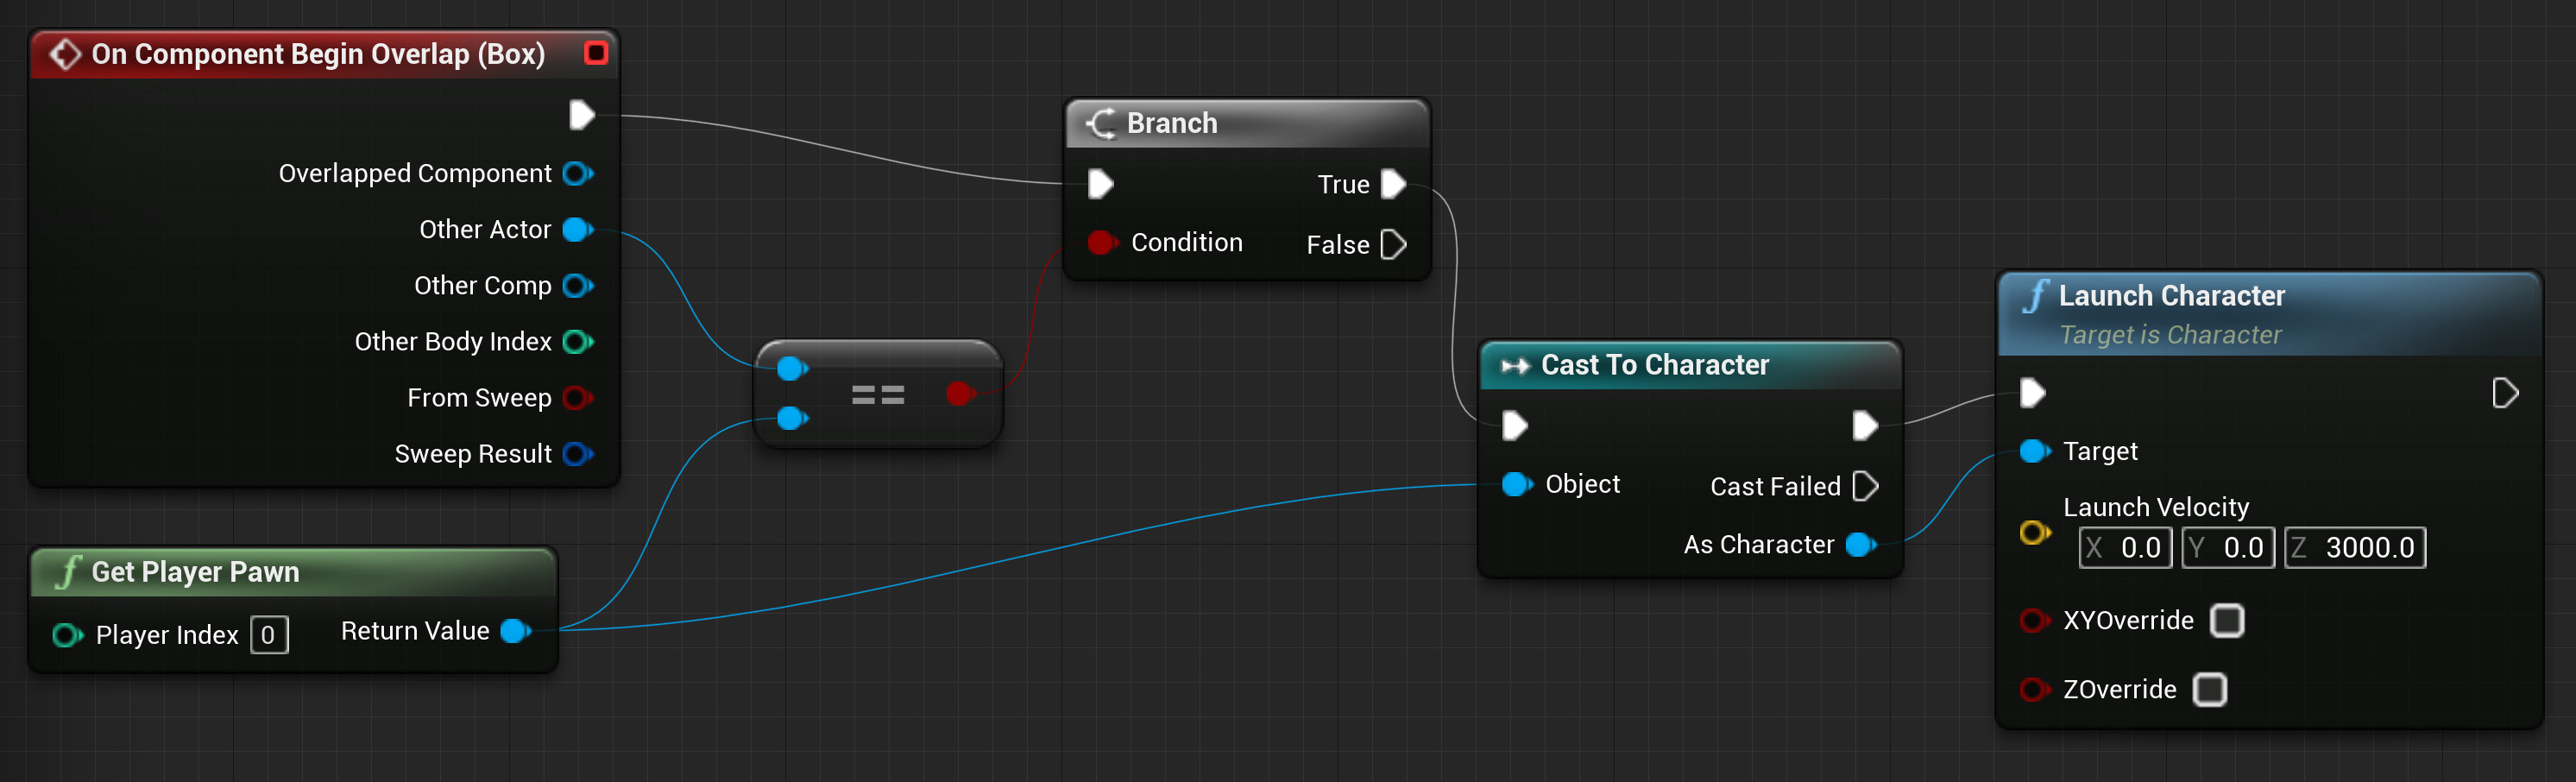
\includegraphics[width=\linewidth]{unreal-blueprints.jpg}
    \caption{}\label{fig:geo-vpl:1}
  \end{subfigure}%
  \qquad %-- that adds some space between th 2 figures
  \begin{subfigure}[b]{0.45\linewidth}
    \graphicspath{{../../assets/images/background/geo-vpl/}}
    \centering
    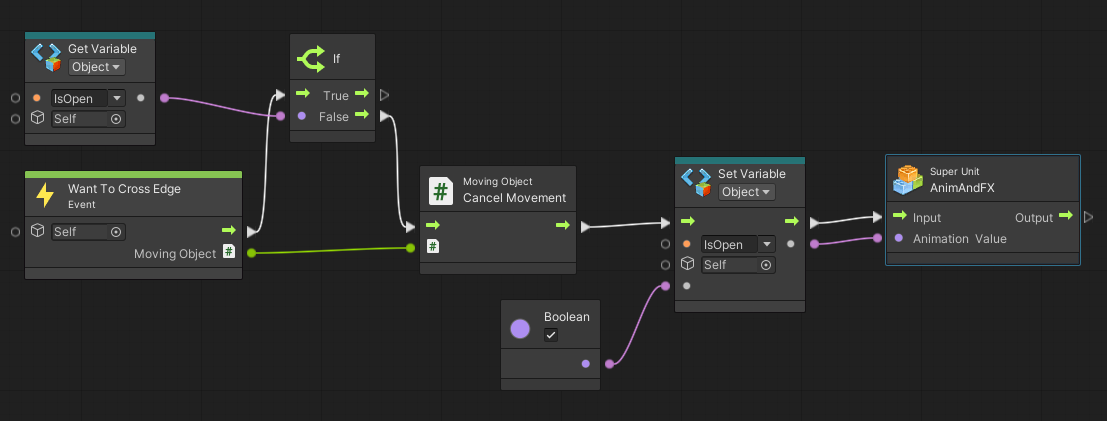
\includegraphics[width=\linewidth]{unity-bolt-2.png}
    \caption{}\label{fig:geo-vpl:2}
  \end{subfigure}%
  \caption[Geometry VPLs]{TODO: add geometry vpls}
  \label{fig:geo-vpl}
  \end{figure}

\subsubsection*{Behavioral VPLs}
The behavioral and logical vpls found in applications such as Unreal's Blueprint and Unity's Bolt (https://docs.unrealengine.com/5.0/en-US/blueprints-visual-scripting-in-unreal-engine/, https://assetstore.unity.com/packages/tools/visual-scripting/bolt-163802) are less relevant to the activity of geocomputation.
However, one interesting property worth mentioning, is that these languages have actually designed a way for end-users to define imperative flow statements, since these could not be overlooked for behavior and logic.
\refsec{sec:background-vpl} named conditions and loops as one of the challenges of diagram-based vpls. 
These languages both attempted to solve this problem by introducing a special "flow state" variable. 
It represents no value, but simply the activity of 'activating' or 'doing' the node selected. 
\reffig{fig:logic-vpl} showcases these flow-state variables in both languages using conditionals.
flow-state variables have their own set of rules, completely separate from connections carrying data. 
For example, they can be used cyclically, offering users looping functionality and are allowed to have multiple sources.  
Despite these functionalities, one might wonder if these aspects are worth these extra complications.
Especially since these flow-state variables are effectively \m{GOTO} statements, which are widely known as an anti-pattern in large-scale software projects. 

\begin{figure}
\centering
\begin{subfigure}[b]{0.45\linewidth}
  \graphicspath{{../../assets/images/background/geo-vpl/}}
  \centering
  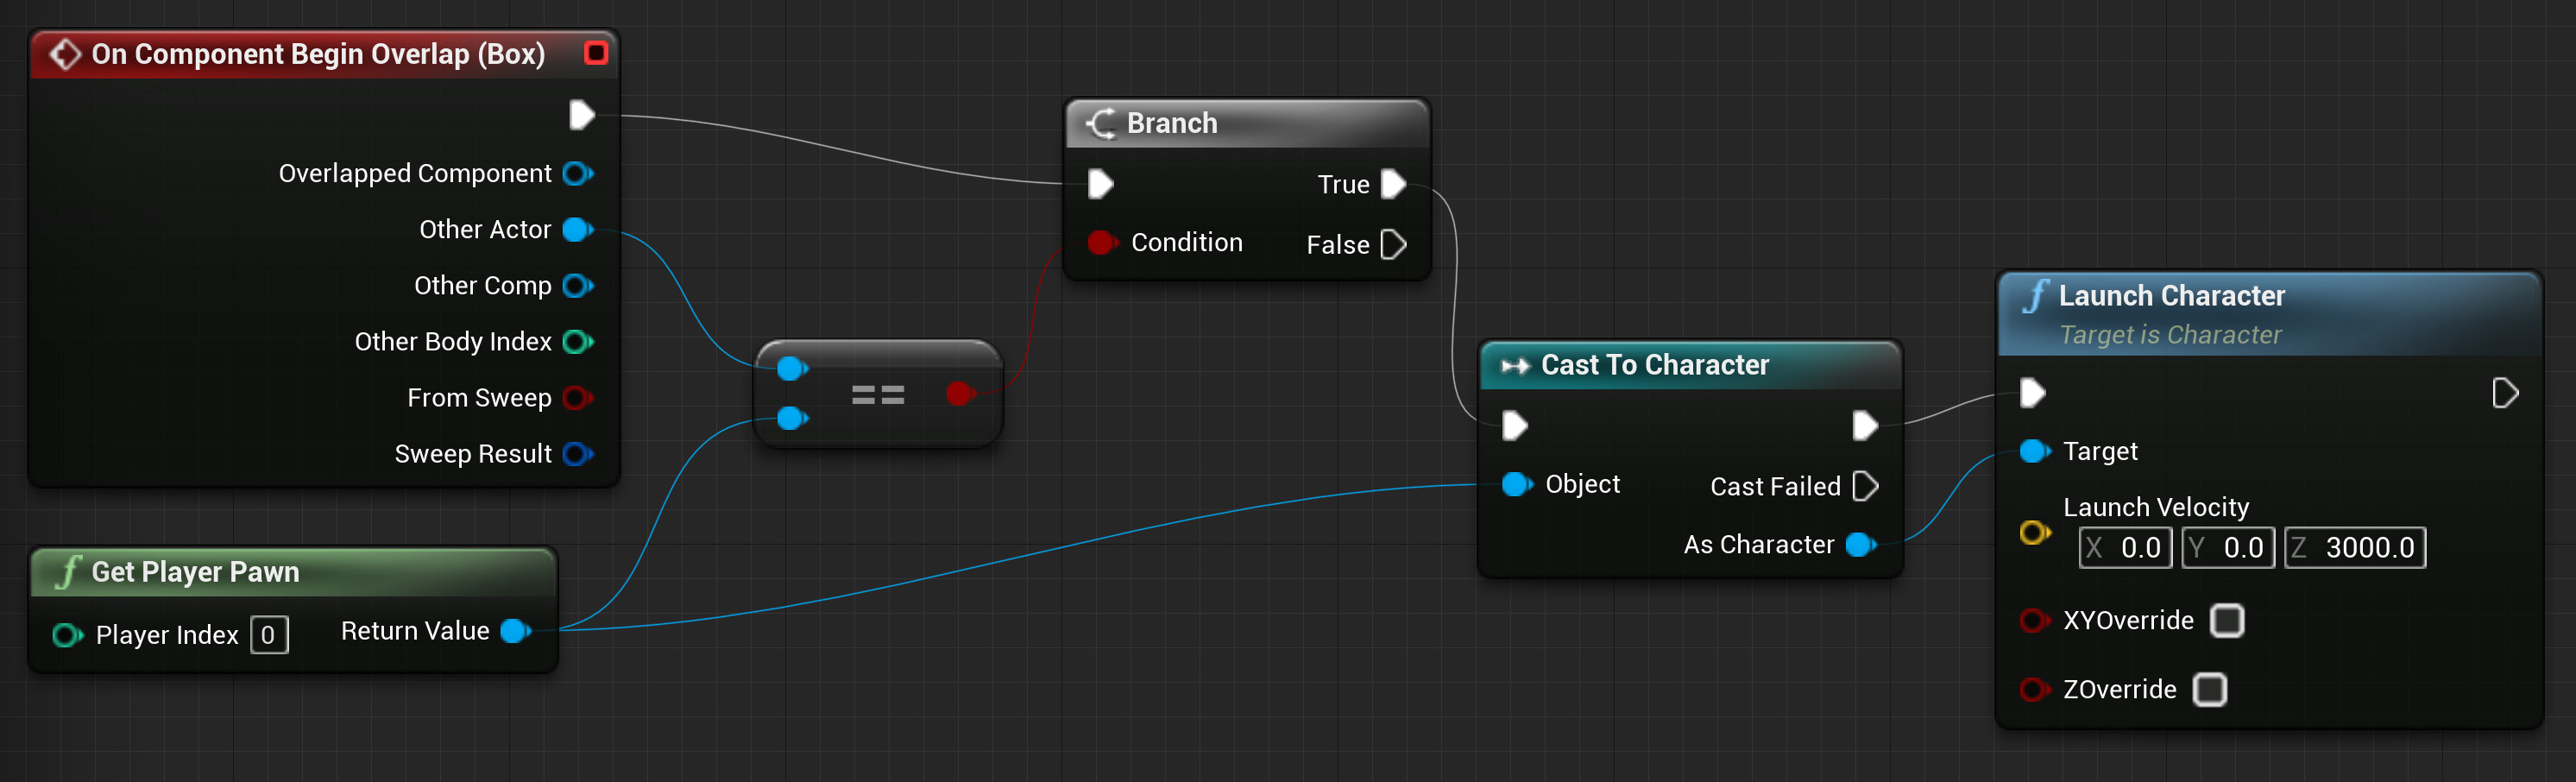
\includegraphics[width=\linewidth]{unreal-blueprints.jpg}
  \caption{}\label{fig:logic-vpl:1}
\end{subfigure}%
\qquad %-- that adds some space between th 2 figures
\begin{subfigure}[b]{0.45\linewidth}
  \graphicspath{{../../assets/images/background/geo-vpl/}}
  \centering
  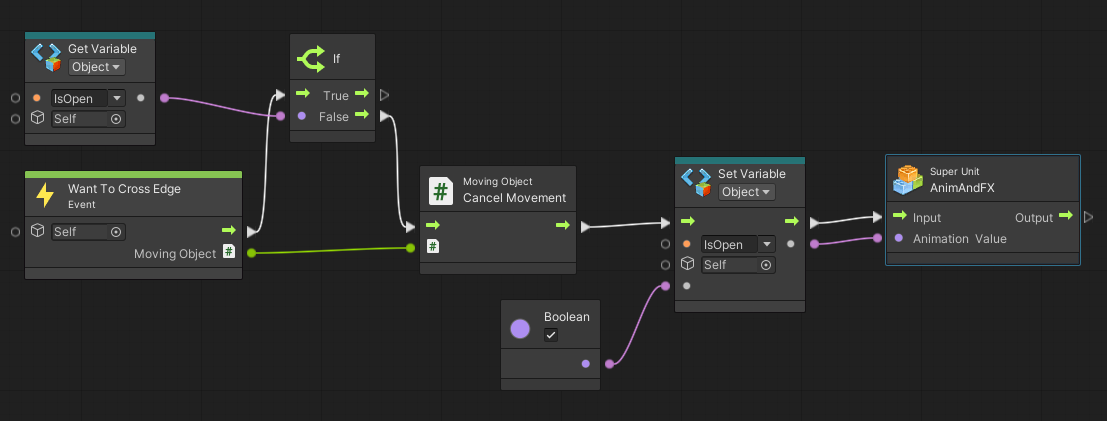
\includegraphics[width=\linewidth]{unity-bolt-2.png}
  \caption{}\label{fig:logic-vpl:2}
\end{subfigure}%
\caption[Behavioral VPLs]{Two behavioral vpls, showing "flow-state" variables. Left: Unreal's Blueprints, Right: Unity's Bolt.}
\label{fig:logic-vpl}
\end{figure}

\section{Browser-based visual programming}
\label{sec:related-webvpl}

This section is dedicated to visual programming applications running in a browser.
It must be emphasized that of all the various vpls named in \refsec{sec:related-geovpl}, none are browser-based. 
This is likely the case because most of those vpls are computationally intensive, C++-based applications.

Nevertheless, if one looks in other domains, we quickly see many \ac{vpl}s which are web-based. 
Out of all 30 VPL studies covered by the meta analysis of \cite{kuhail_characterizing_2021}, 17 were web based, 7 were mobile based, and only 6 were desktop applications. 
Kuhail et al. continue by noting that most of these 6 desktop applications were build during or before 2013. 
The reason Kuhail et al. present for this stark difference is completely in one line with \refsec{sec:background-web}: 
\emph{"This can be explained by the fact that desktop-based tools are cumbersome to contemporary users. They must be downloaded and installed, are operating-system dependent, and need frequent updates."}.

\begin{figure}
\centering
\begin{subfigure}[b]{0.45\linewidth}
  \graphicspath{{../../assets/images/background/web-vpl/}}
  \centering
  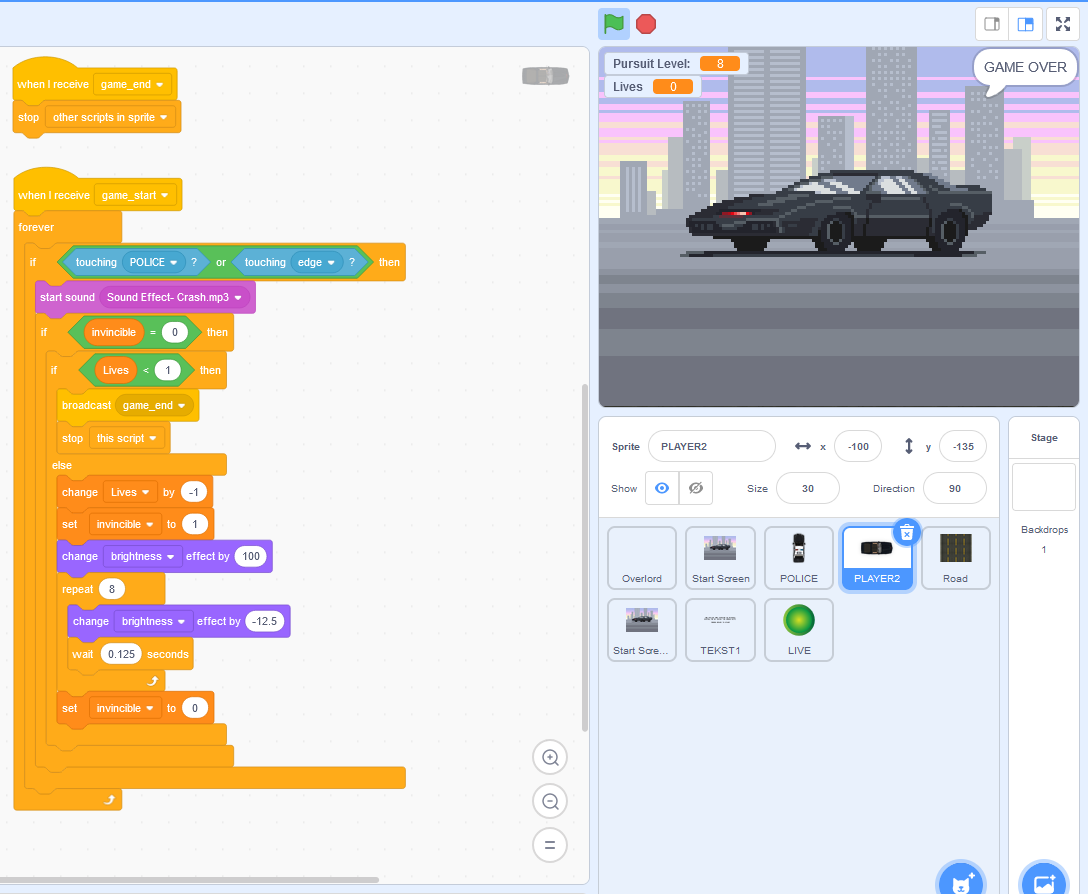
\includegraphics[width=\linewidth]{scratch-2.png}
  \caption{}\label{fig:webvpl:1}
\end{subfigure}%
\qquad 
\begin{subfigure}[b]{0.45\linewidth}
  \graphicspath{{../../assets/images/background/web-vpl/}}
  \centering
  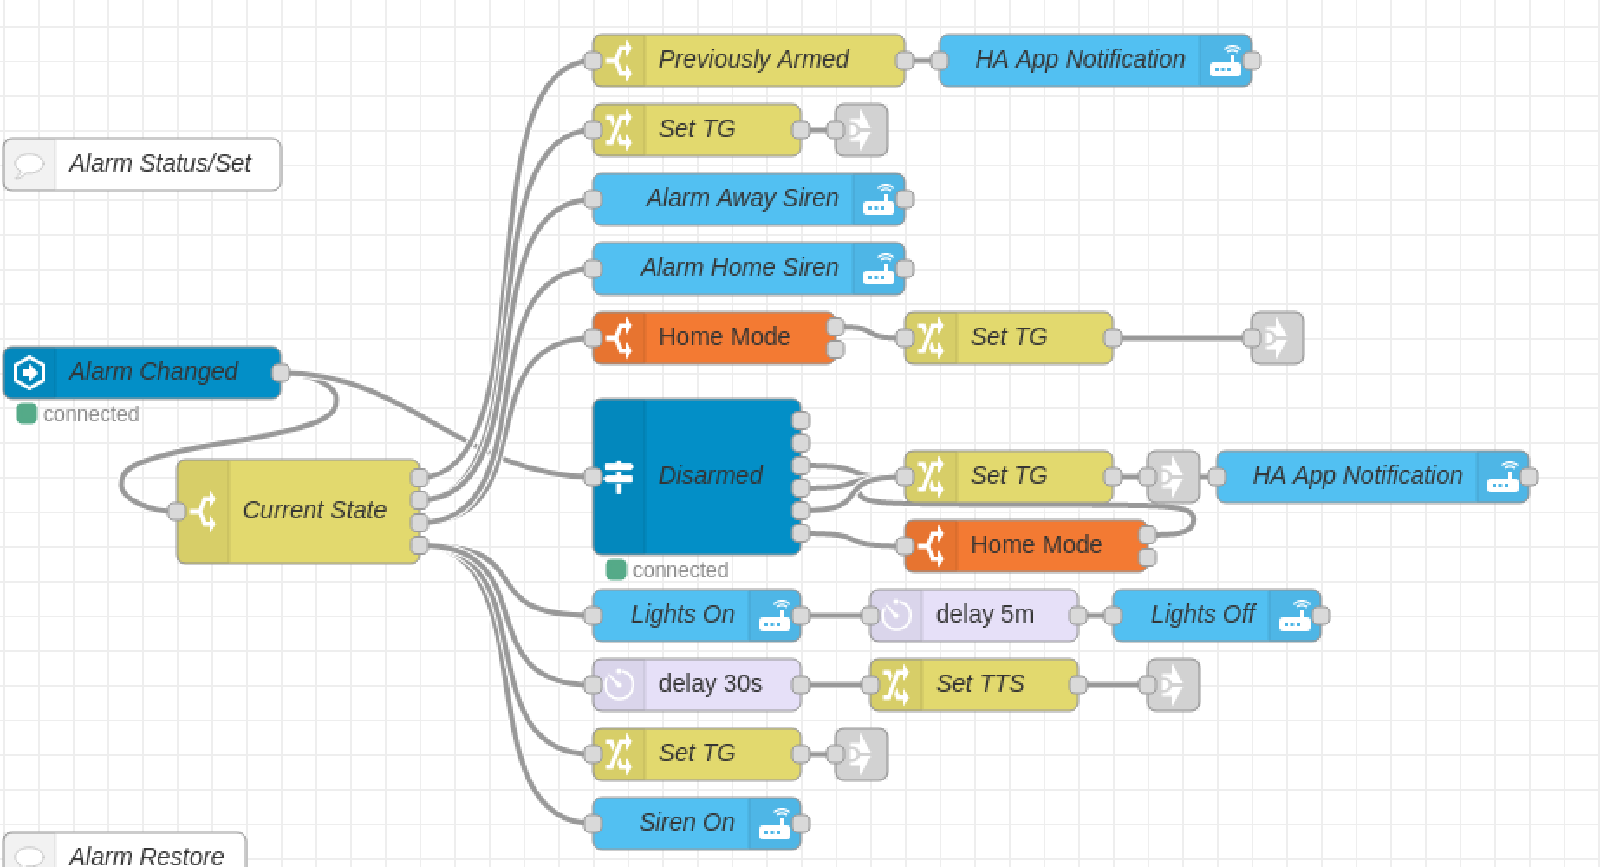
\includegraphics[width=\linewidth]{nodered-2.png}
  \caption{}\label{fig:webvpl:2}
\end{subfigure}%
\caption[web VPLs]{Two VPLs used on the web: Scratch (a), and nodeRED (b). }
\label{fig:webvpl}
\end{figure}

% (SOURCE: https://dl.acm.org/doi/fullHtml/10.1145/1592761.1592779?casa_token=cJ1iX1YYimkAAAAA:YVyp3KFiKwD2GMuBUUIgvibbNsEgndqNQzehRnCosCpyEx51C_uNpi2D4-lsE-x88hQFSWcbTfrP_w)
% (https://www.ucode.com/coding-classes-for-kids/is-scratch-the-same-as-blockly)
% (https://developers.google.com/blockly/)
% (https://developers.googleblog.com/2019/01/scratch-30s-new-programming-blocks.html)
This study wishes to present two web based visual programming languages, which each use the web in a meaningful way.  
The first web-vpl is "Scratch", and Googles related "Blockly" project (Source, See \reffig{fig:webvpl:1}). 
Scratch is well-known as an educational, block-based vpl, targeted at children and young adults to teach the basics of computational thinking. 
The program is famously used as the first assignment of Harvard university's CS50 course (Source: https://www.youtube.com/watch?v=1tnj3UCkuxU).   
As noted by the authors of CS50, scratch is, despite this target audience, surprisingly close to any normal programming language, with for and while loops, if statements, and even event handling and asynchronous programming. 
Scratch used to be a desktop application. 
The web environment this vpl now occupies allows its users excellent life-cycle support. 
Users can immediately publish their work, search for and run the work of others, and even "Remix / clone / fork" the source code of these other projects. 
This encourages users to learn from each other.

[blockly-> can be compiled to python and javascript]
Microsoft makecode arcade


The second exemplary web vpl this study wishes to bring to the readers attention is the "nodeRED" application (Source, see \reffig{fig:webvpl:2}). 
This is a feature-rich diagram-based application, created to serve the domain of IoT.
This vpl uses the browser-based platform not only for the aforementioned \refsec{sec:background-web} reasons, but also for the exact same reasons a router, NAS or IoT device often opts for a browser-based interface: 
Servers, either small or big, explaining how they desire to be interfaced, is more or less the cornerstone all web clients are based upon.  
If the server serves its corresponding client, users do not need to find some compatible interface themselves.
For this reason the "nodeRED" application is a web application, even though it is mostly run on local networks.   

\section{Browser-based Visual programming and geocomputation} 

% - Mobius Modeller : https://mobius.design-automation.net/pages/mobius_modeller.html
To the best of the author's knowledge, only one publicly available visual programming language exist which is both able to be configured and executed in a browser, and is able to be used for geodata computation.
This application is called the Möbius modeller (Source: https://mobius-08.design-automation.net/about), and is by far the closest equivalent to the geo-web-vpl proposed by this study.
Though it only uses javascript, the tool is able to be successfully used for an impressive range of applications, including CAD, BIM, urban planning, and GIS. 
It uses a combination of a very 'bare-bones' diagram-based vpl, together with a very rich block-based vpl (See \reffig{fig:mobiusmodeller}).
In fact, the block-based vpl is so rich that is almost ceases to be a vpl altogether, and starts to be python-like language with heavy IDE support.  

The \ac{geo-web-vpl} presented by this study still differs from the mobius modeller in the following aspects: 
\begin{itemize}[-]
  \item This study explores the usage of diagram-based vpls as opposed to a block-based vpl, to allow for the dataflow programming advantages described in \refsec{sec:background:dataflow}.
  \item This study explores the usage of WebAssembly to hypothetically improve performance and to use existing geocomputation libraries.
  \item This study addresses some of the life-cycle issues of \ac{vpl}s stated in \refsec{sec:background:vpl:disadvantages}. 
\end{itemize}

\begin{figure}
  \centering
  \begin{subfigure}[b]{0.45\linewidth}
    \graphicspath{{../../assets/images/background/geo-web-vpl/}}
    \centering
    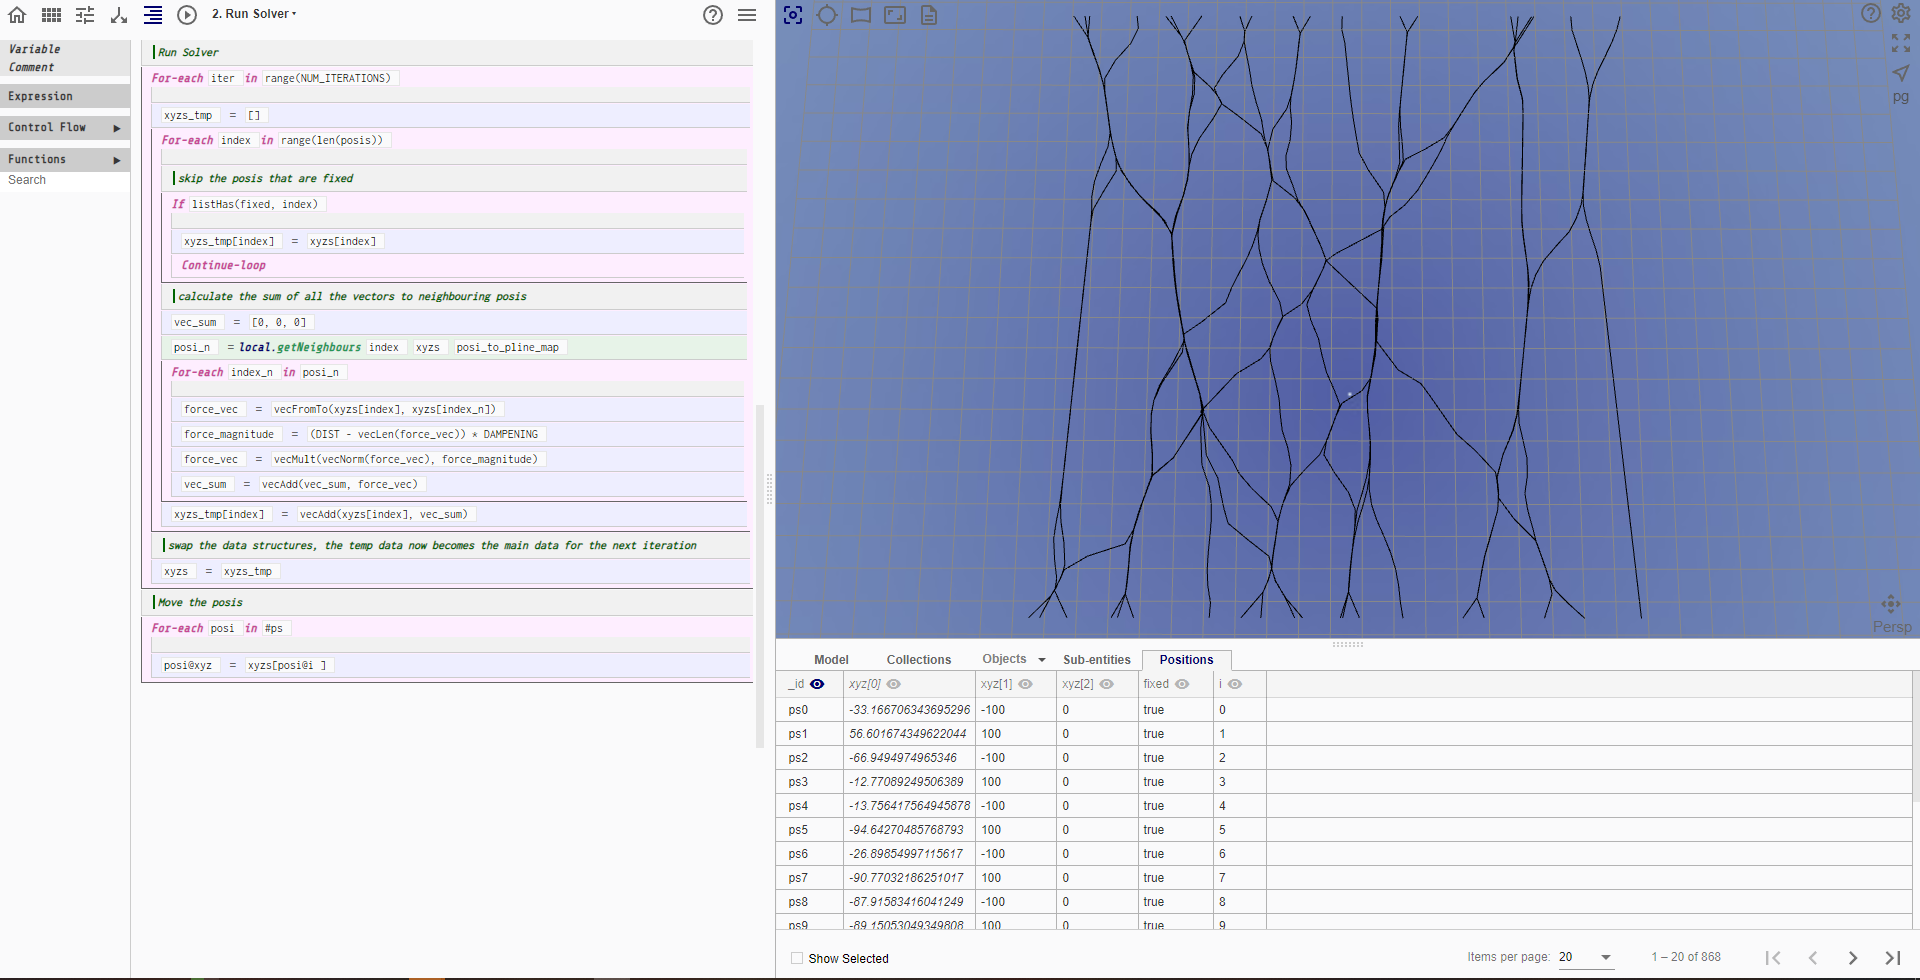
\includegraphics[width=\linewidth]{mobius-3.png}
    \caption{}
  \end{subfigure}%
  \qquad %-- that adds some space between th 2 figures
  \begin{subfigure}[b]{0.45\linewidth}
    \graphicspath{{../../assets/images/background/geo-web-vpl/}}
    \centering
    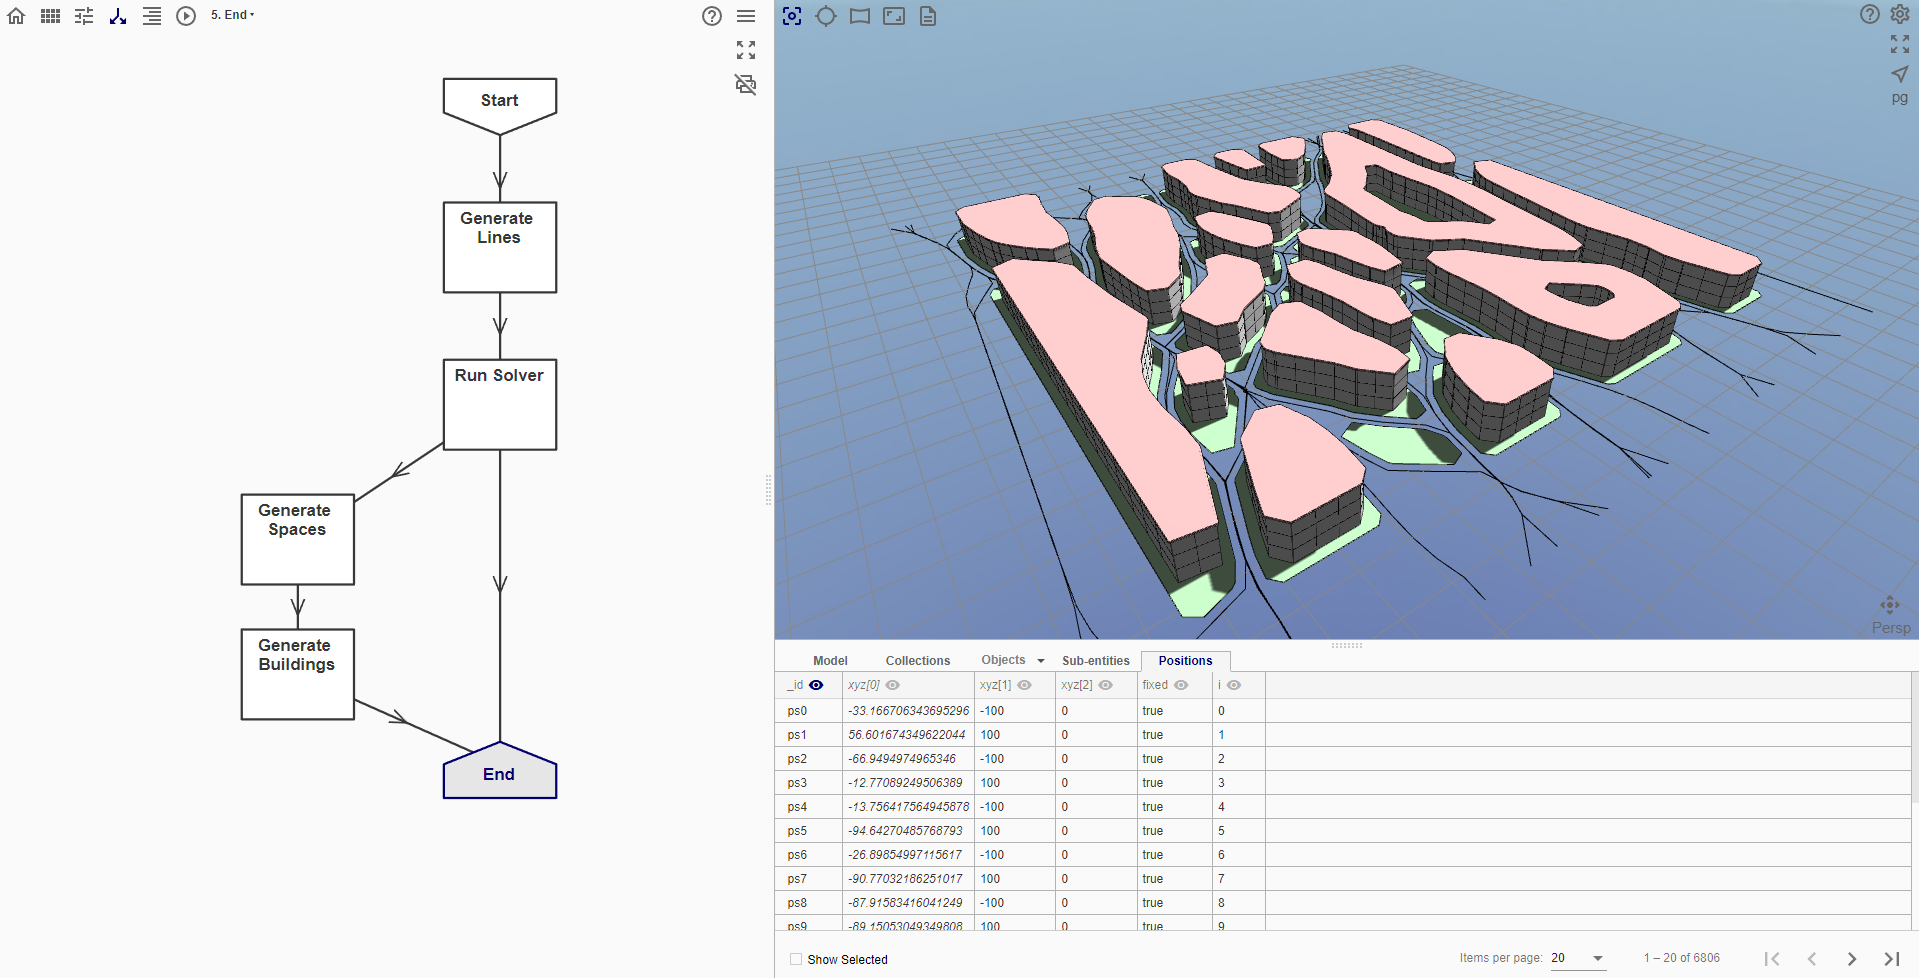
\includegraphics[width=\linewidth]{mobius-4.png}
    \caption{}
  \end{subfigure}%
  \caption[Mobius Modeller]{Images of the Mobius modeller application}%
  \label{fig:mobiusmodeller}
  \end{figure}

%% SOME THOUGHTS ON RELATED WORKS: 

% GEO: the thing we want to do
% VPL: best choice for end user development, 
% WEB: solves the huge life-cycle problem of publication


% SOME THOUGHTS ABOUT THE IMPORTANCE OF EXPERIMENTATION AND PLAY
% -> testing & reproducability.
% RANSAC -> many 'magic' parameter. 
% Game Of Life -> impossibility of 'proving' behaviour systems. 
% Many parameters simply need to be discovered by 'play' / simulation
% Jonathan blow -> using interactive applications, an intrinsic understanding can be gained without explicit communication.

% gdevelop 